The primary interface to the PFA is through a number of memory-mapped queues:
\gls{freeq}, \gls{newq}, and \gls{evictq}. The \gls{freeq} contains unused page
frames that the PFA can use for fetching new pages, the \gls{newq} reports any
recently fetched pages to the OS bookkeeping thread, and the \gls{evictq}
contains a list of local pages that should be stored in remote memory. Using
these queues, execution proceeds as follows:

\paragraph{Eviction}
The PFA handles all communication with the memory blade. This includes page
eviction. The basic procedure is as follows (see figure \ref{fig:evict_detail}):

\begin{outline}[enumerate]
    \1 The OS identifies pages that should be stored remotely.
    \1 It evicts them explicitly by writing to the \gls{evictq}.
    \1 The PFA sends a remote memory write command to the NIC which reads the
    page through DMA and sends it to remote memory.
    \1 When the send is complete, the PFA updates the \gls{evictq} status to
    notify the OS.
    \1 The OS stores a page identifier in the PTE and marks it as remote once
    the PFA eviction is complete.
\end{outline}

\begin{figure}[h] \centering
  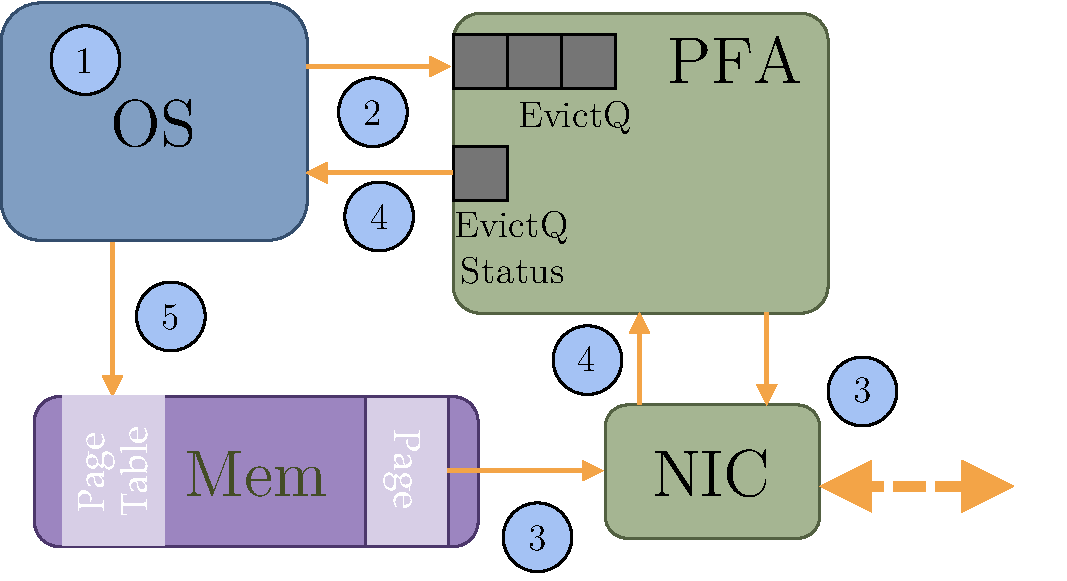
\includegraphics[width=0.7\columnwidth]{figs/pfa_evict_detail.pdf}
  \caption{Detailed eviction flow}
  \label{fig:evict_detail}
\end{figure}

In addition to the three main queues, there are a number of other maintenance
registers that are used for querying queue status and initializing the PFA. I
will mention one status register here; the EVICT\_STAT register. When a page is
placed on the evict queue, the PFA begins transferring it to remote memory, but
does not block the OS. This allows the OS to perform useful work while the
eviction is taking place, potentially hiding some of the write latency. In
order to re-use the page frame, however, the OS must poll the EVICT\_STAT
register to ensure the write has completed.

\paragraph{Fetch}
The primary function of the PFA is to automatically fetch pages from remote
memory when an application tries to access it. It does this by detecting page
table entries that are marked remote and transparently re-mapping them to the
next available free frame. The basic operation is as follows (see figure
\ref{fig:fetch_detail}):

\begin{outline}[enumerate]
    \1 Application code issues a load/store for the (now remote) page.
    \1 The TLB and PTW detect a remote page and request it from the PFA
    \1 The PFA issues a remote memory read command to the NIC, providing the
    next available frame from the \gls{freeq}.
    \1 The PFA clears the remote bit in the \gls{pte}.
    \1 The PFA pushes the virtual address of the fetched page to the NewQ.
    \1 The application is restarted.
\end{outline}

\begin{figure}[h] \centering
  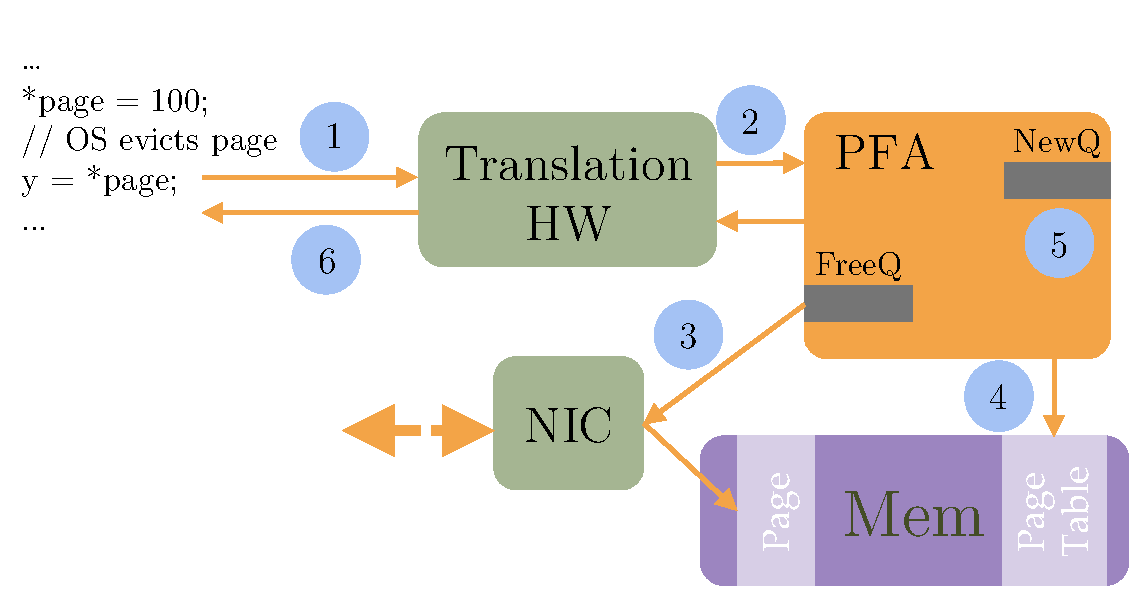
\includegraphics[width=0.8\columnwidth]{figs/pfa_fetch_detail.pdf}
  \caption{Detailed fetch flow}
  \label{fig:fetch_detail}
\end{figure}
\FloatBarrier

\paragraph{Metadata Management}
The OS should ensure that there are sufficient free frames in the \gls{freeq} to
ensure smooth operation. If a remote page is requested and there are no free
frames, the PFA will trap to the OS with a conventional page-fault. The OS must
enqueue one or more free-frames before returning from the interrupt. This may
involve evicting pages synchronously in the page-fault handler.

Similarly, the OS needs to drain the new page queue periodically to ensure it
does not overflow. This will also trap to the OS with a conventional page
fault.

% \subsubsection{Page Table Entry} \label{sec:remPTE}
% The PFA uses a special PTE format for remote pages (Figure
% \ref{fig:pte_format}). The fields are as follows:
%
% \begin{outline}
%   \1 \textbf{\gls{pgid}}: This acts as an address in remote memory for the remote
%   page. It is used by the PFA to look up pages in remote memory, and for the OS
%   to identify each page during bookkeeping.
%   \1 \textbf{Prot}: This sets the protection bits that the PFA will use when
%   fetching a page. These bits include things like read/write permissions, as
%   well as other page metadata (see the RISC-V privileged architecture manual
%   for more details \cite{riscv_priv110}).
%   \1 \textbf{R}: This bit indicates that a page is remote (when the valid bit
%   is clear).
%   \1 \textbf{V}: This indicates whether a page is valid.  A valid page is
%   currently in main memory and would not trigger a page-fault.  This is also
%   referred to as the ``present bit'' in Linux.
% \end{outline}
%
% \begin{figure}[h]
%   \centering
%   \begin{bytefield}[endianness=big,bitwidth=0.015\linewidth]{64}
%     \bitheader{0, 1, 2, 12, 40, 63} \\
%     \bitbox{24}{Unused} & \bitbox{28}{Page ID} & \bitbox{10}{Prot} &
%     \bitbox{1}{\tiny R} & \bitbox{1}{\tiny V} \\
%   \end{bytefield}
% 	\caption{Remote PTE Format. The \textbf{Page ID} is a unique identifier of this page
%   and serves as a remote memory address. The \textbf{Prot} field contains the permission
% and metadata bits that should be set after a page is fetched (see the RISC-V
% specification for details\cite{riscv_priv110}). The \textbf{R} bit indicates
% that this page is remote while the \textbf{V} bit indicates that the PTE is not
% a valid mapping (needed for backward compatibility).}
% 	\label{fig:pte_format}
% \end{figure}
%
% An interesting feature of this design is the use of pre-defined protection
% bits. This includes a valid bit which can be cleared by the OS before evicting
% to trigger a page fault on this page immediately after fetching (a useful
% debugging feature). Also, bits 8 and 9 are reserved for software by the RISC-V
% ISA and can aid the OS in bookkeeping and debugging (see Section
% \ref{sec:linuxImpl}).
%
\subsubsection{Remote Memory Interface}
The PFA requires some hardware-accessible interface to remote memory. This
could be through a memory semantic fabric or RDMA-enabled network (such as
Infiniband or RoCE). In our design, we use a custom implementation of RDMA over
ethernet to a dedicated memory blade. This interface is accessible to both
software (through a Linux driver) and the PFA (through an on-chip network).

